\chapter{RESULTADOS}
\label{cap:resultados}

Este capítulo sigue la estructura del Capítulo~\ref{cap:metodo}, como se
indica al inicio de ese capítulo. Las Unidades~1 y~2 se ejecutaron sobre
escaneos reales de la Catedral de Lima; su propósito no es demostrar que el
sistema acierta, porque todavía no hay etiquetas con las que medirlo, sino que el
procedimiento escrito es ejecutable y reproducible. Solo se reporta lo
ejecutado; lo que aún no se ha ejecutado se indica en una línea.

% =====================================================================
\FloatBarrier
\section{Diagrama de Flujo General}
\label{sec:res-flujo}

Responde a la Sección~\ref{sec:diagrama-flujo}. De las etapas de la
Figura~\ref{fig:flujo} se han ejecutado E0, E1 y E2 (Tabla~\ref{tab:res-etapas});
E3 a E5 y el bucle de repeticiones aún no.

\begin{table}[!htbp]
\centering
\setstretch{1}\small
\caption[Etapas ejecutadas del flujo general]{Etapas ejecutadas del flujo general y sección donde está su resultado. Elaboración propia.}
\label{tab:res-etapas}
\begin{tabularx}{\linewidth}{@{}l>{\raggedright\arraybackslash}Xl@{}}
\toprule
\textbf{Etapa} & \textbf{Alcance ejecutado} & \textbf{Resultado} \\
\midrule
E0 & Recepción de los 23 archivos LAS, sin etiquetas & \S\ref{sec:res-u1-datos} \\
E1 & Preprocesamiento de las 23 secciones & \S\ref{sec:res-u1-repro} \\
E2 & Extracción con Sonata sobre PL13 & \S\ref{sec:res-unidad2} \\
\bottomrule
\end{tabularx}
\end{table}

La frontera de disco funciona en un sentido: el archivo \texttt{.npz} de PL13 se
escribió desde el entorno de Sonata y el visor lo leyó fuera de él. Falta que lo
lea el entorno de HyperNCD.

% =====================================================================
\FloatBarrier
\section{Hardware y Repositorio}
\label{sec:res-hardware}

Responde a la Sección~\ref{sec:hardware-repo}. Las pruebas de la Unidad~1 sobre
PL13 y PL7 corrieron en la laptop local; el preprocesamiento de las 23 secciones
y la extracción con Sonata, en Khipu, esta última en una RTX~A6000 de 48\,GB.
Todas se lanzaron con los programas y guiones del repositorio y las órdenes del
\hyperref[sec:anexo-software]{Anexo~A}. Los tiempos de cada una están en su unidad.

% =====================================================================
\FloatBarrier
\section{Diseño General del Sistema}
\label{sec:res-diseno}

Responde a la Sección~\ref{sec:diseno}.

\FloatBarrier
\subsection{Estructura y Contrato de los Módulos}
\label{sec:res-contrato}

Las salidas de los Módulos~1 y~3 tienen la forma que declara la
Tabla~\ref{tab:contrato}: la matriz $S$ de 9 columnas
(Tabla~\ref{tab:m1-metadatos}) y $f_{\mathrm{ssl}}$ de 1088 valores en la
rejilla de 2\,cm, con un índice inverso de una entrada por fila de $S$
(Tabla~\ref{tab:npz}). Los Módulos~2, 4 y~5 aún no se han ejecutado.

\FloatBarrier
\subsection{Visor 3D del Proyecto}
\label{sec:res-visor}

Al dibujar los descriptores de PL13 (Figura~\ref{fig:visor-pl13-etapas}), el
visor verificó que el archivo \texttt{.npz} corresponde a la matriz $S$ de la que
salió.

% =====================================================================
\FloatBarrier
\section{Unidad 1. Preprocesamiento}
\label{sec:res-unidad1}

Responde a la Sección~\ref{sec:unidad1}.

\FloatBarrier
\subsection{Datos de Entrada y Ejecución}
\label{sec:res-u1-datos}

El procedimiento se ejecutó sobre dos escaneos de la Catedral de Lima, PL13 y
PL7, en el equipo local de la Sección~\ref{sec:hardware-repo}. PL13 es el
escaneo principal, porque es el que después pasa por Sonata en la
Sección~\ref{sec:res-unidad2}, de modo que todo el análisis sigue al mismo
escaneo de principio a fin. PL7 se presenta al lado como segundo ejemplo, para
mostrar que el procedimiento se comporta igual en otro escaneo. PL13 es el
1{,}40\,\% del levantamiento y PL7 el 1{,}46\,\%.

Las dos pruebas usaron los valores por defecto de la
Sección~\ref{sec:u1-procedimiento} (Tabla~\ref{tab:m1-metadatos}).
Las figuras de nubes de esta sección dibujan 200\,000 puntos tomados al azar,
salvo donde se indique.


\FloatBarrier
\subsection{Procedimiento}
\label{sec:res-u1-procedimiento}

Cada paso responde al paso del mismo número de la
Sección~\ref{sec:u1-procedimiento}.

\FloatBarrier
\subsubsection*{Paso 1. Carga}

Cada escaneo se lee en dos bloques, en cerca de un segundo (\texttt{n\_crudo}
en la Tabla~\ref{tab:m1-metadatos}). Es la data de entrada tal como la entrega el
escáner, con su color real y sin ninguna corrección
(Figura~\ref{fig:m1-paso1}).

\begin{figure}[!htbp]
\centering
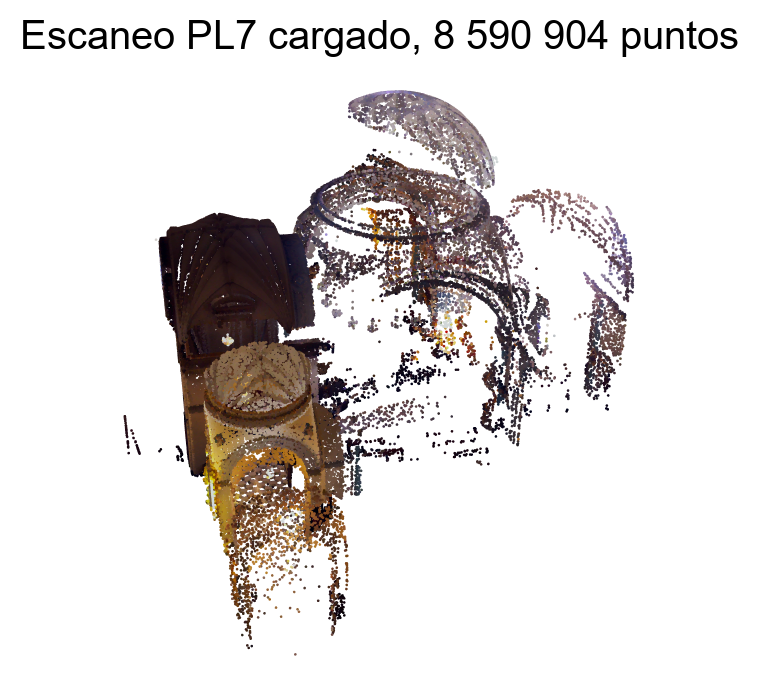
\includegraphics[width=0.75\linewidth]{imagenes/m1_paso1_carga.png}
\caption[PL13 y PL7 tras la carga]{PL13 y PL7 tras la carga. Elaboración propia con el visor del proyecto (\hyperref[sec:anexo-software]{Anexo~A}).}
\label{fig:m1-paso1}
\end{figure}

\FloatBarrier
\subsubsection*{Paso 2. Centrado}

Los dos escaneos son vecinos, sus centros están a unos 17\,m uno de otro, pero
cada uno se centra en su propio origen (Tabla~\ref{tab:m1-centrado}). Este paso no lleva imagen
porque la nube se ve igual antes y después, solo cambian los números de los
ejes.

\begin{table}[!htbp]
\centering
\setstretch{1}\small
\caption[Coordenadas de PL13 y PL7 antes y después del centrado]{Coordenadas de PL13 y PL7 antes y después del centrado, en metros. Elaboración propia.}
\label{tab:m1-centrado}
\begin{tabularx}{\linewidth}{@{}ll>{\raggedright\arraybackslash\hsize=1.00\hsize}Xll@{}}
\toprule
\textbf{Escaneo} & \textbf{Eje} & \textbf{Antes, en UTM} & \textbf{Centro} & \textbf{Después} \\
\midrule
PL13 & $x$ & 278\,772{,}08 a 278\,804{,}90 & 278\,788{,}49 & $-16{,}41$ a $16{,}41$ \\
     & $y$ & 8\,667\,747{,}60 a 8\,667\,779{,}68 & 8\,667\,763{,}64 & $-16{,}04$ a $16{,}04$ \\
     & $z$ & 161{,}61 a 183{,}89 & 172{,}75 & $-11{,}14$ a $11{,}14$ \\
\midrule
PL7  & $x$ & 278\,775{,}30 a 278\,826{,}64 & 278\,800{,}97 & $-25{,}67$ a $25{,}67$ \\
     & $y$ & 8\,667\,724{,}83 a 8\,667\,780{,}02 & 8\,667\,752{,}42 & $-27{,}60$ a $27{,}60$ \\
     & $z$ & 159{,}36 a 188{,}83 & 174{,}10 & $-14{,}73$ a $14{,}73$ \\
\bottomrule
\end{tabularx}
\end{table}

\FloatBarrier
\subsubsection*{Paso 3. Filtrado SOR}

En PL13 se descartan 219\,108 puntos, el 2{,}66\,\%, y en PL7 406\,485, el
4{,}73\,\% (\texttt{n\_sor} en la Tabla~\ref{tab:m1-metadatos}). El filtrado tardó
cerca de nueve segundos en PL13 y doce en PL7.

En ambos escaneos los descartes se concentran en las zonas ralas, lejos del
escáner (Figura~\ref{fig:m1-paso3}). PL7
descarta casi el doble que PL13, y en la figura se ve que también tiene más
zonas ralas.

\begin{figure}[!htbp]
\centering
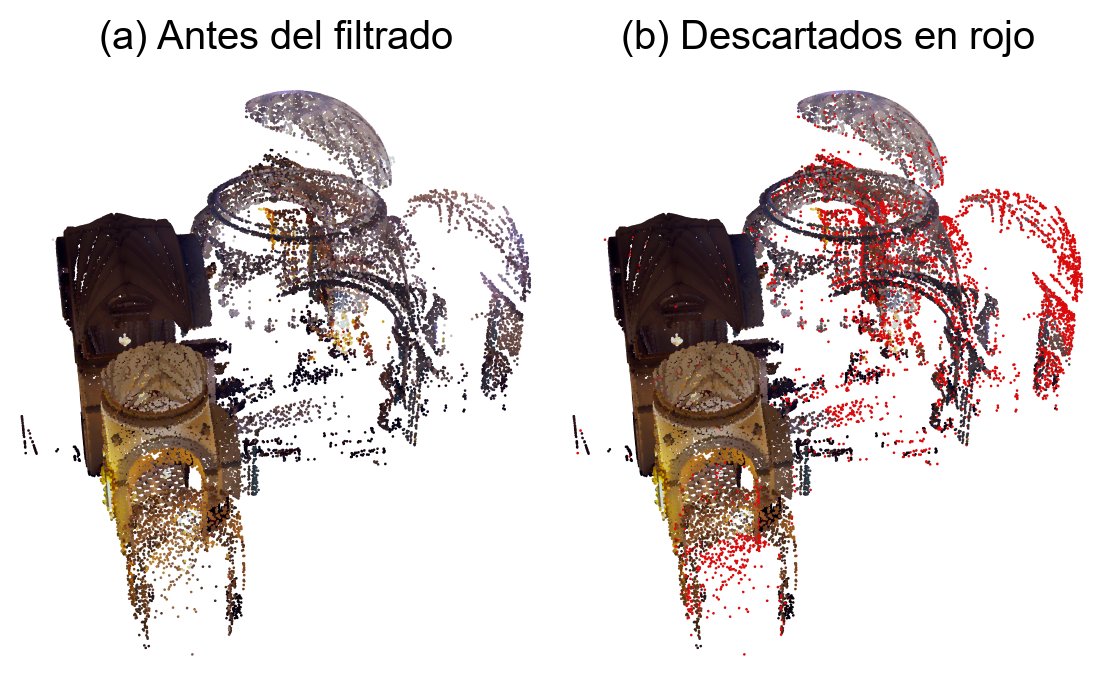
\includegraphics[width=0.85\linewidth]{imagenes/m1_paso3_sor.png}
\caption[PL13 y PL7 con los puntos descartados por el SOR en rojo]{PL13 y PL7 con los puntos descartados por el SOR en rojo. Elaboración propia con el visor del proyecto (\hyperref[sec:anexo-software]{Anexo~A}).}
\label{fig:m1-paso3}
\end{figure}

\FloatBarrier
\subsubsection*{Paso 4. Voxelización}

En PL13 quedan como representantes el 10{,}01\,\% de los puntos que salieron
del filtrado, y en PL7 el 7{,}46\,\% (\texttt{n\_voxel} en la
Tabla~\ref{tab:m1-metadatos})
(Figuras~\ref{fig:m1-paso4-pl13} y~\ref{fig:m1-paso4}). De cerca
(Figuras~\ref{fig:cubo-pl13} y~\ref{fig:cubo-pl7}), en el cubo de PL13 los
37\,777 puntos de la entrada quedan en 1\,159 representantes, y en el de PL7 los
48\,098 quedan en 921. En el cubo de PL7 la entrada contiene varias superficies
paralelas separadas por pocos centímetros, que en la salida ya no se distinguen,
como anticipa el \enlace{sec:u1-p4}{Paso~4}. En los cubos se dibujan todos los puntos, con el color aclarado por un
factor de 2{,}2. Los dos cubos se eligieron con el mismo criterio, tener muchos
puntos y superficies en varias orientaciones. El de PL13 va de $x=-3$ a $-2$\,m,
de $y=7$ a $8$\,m y de $z=-8$ a $-7$\,m, y el de PL7 de $x=-19$ a $-18$\,m, de
$y=-3$ a $-2$\,m y de $z=-12$ a $-11$\,m, en las coordenadas centradas de cada
escaneo.

\begin{figure}[!htbp]
\centering
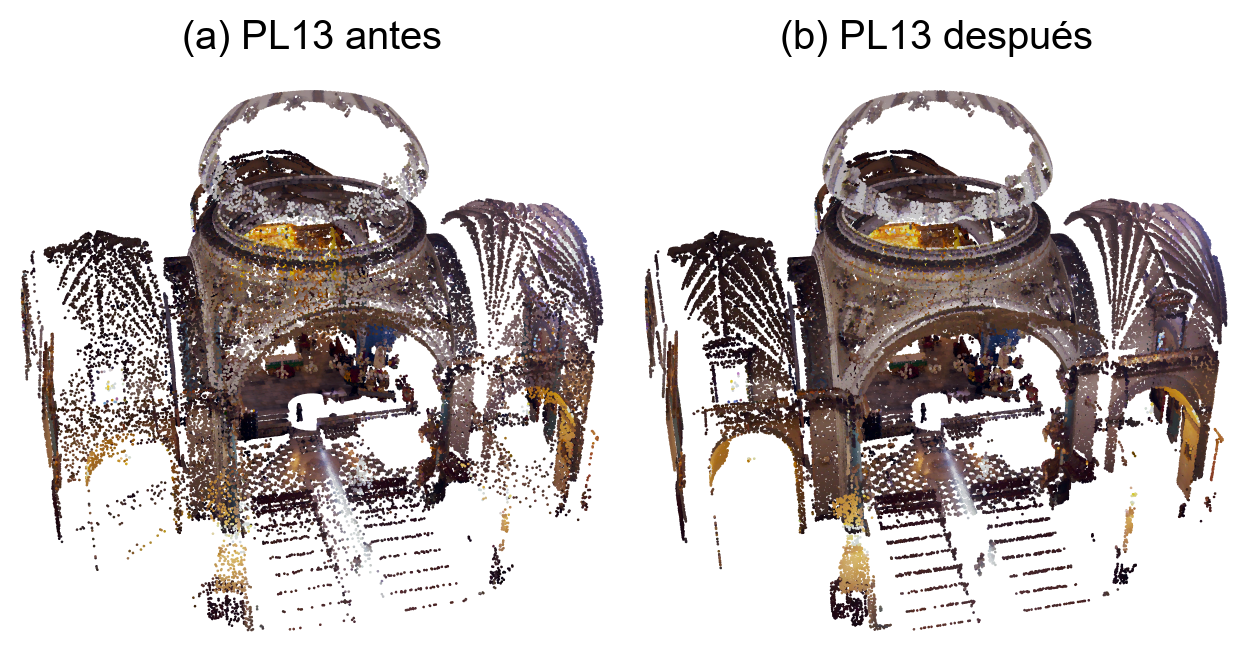
\includegraphics[width=0.75\linewidth]{imagenes/m1_paso4_voxel_completo_pl13.png}
\caption[PL13 antes y después de la voxelización]{PL13 antes y después de la voxelización. Elaboración propia con el visor del proyecto (\hyperref[sec:anexo-software]{Anexo~A}).}
\label{fig:m1-paso4-pl13}
\end{figure}

\begin{figure}[!htbp]
\centering
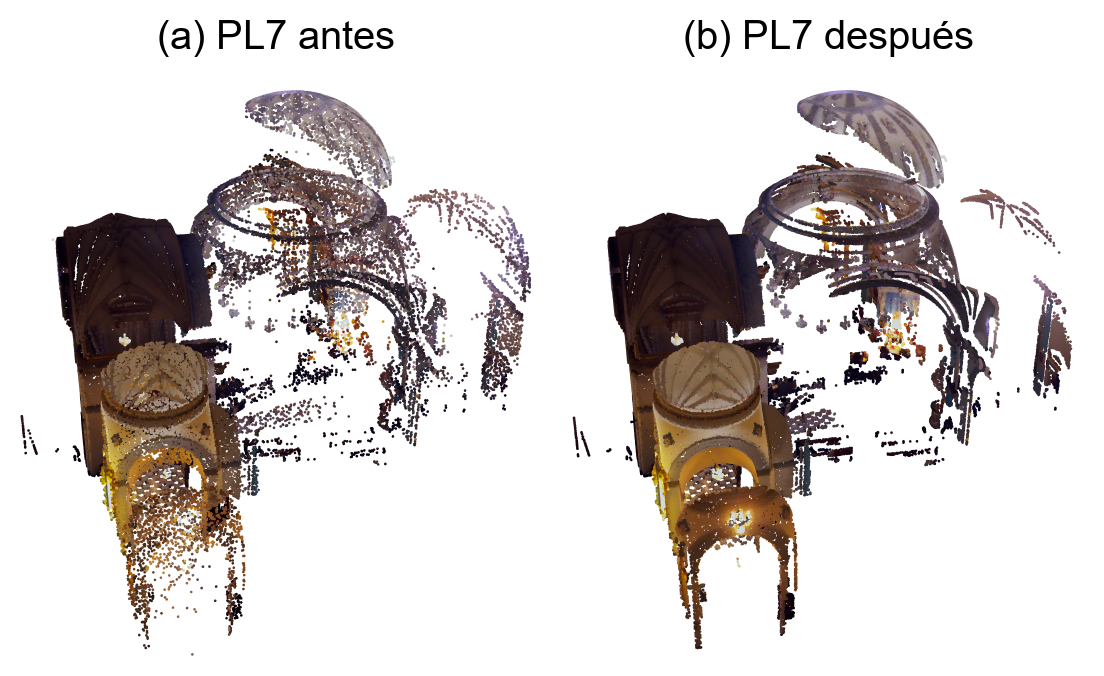
\includegraphics[width=0.75\linewidth]{imagenes/m1_paso4_voxel_completo.png}
\caption[PL7 antes y después de la voxelización]{PL7 antes y después de la voxelización. Elaboración propia con el visor del proyecto (\hyperref[sec:anexo-software]{Anexo~A}).}
\label{fig:m1-paso4}
\end{figure}

\begin{figure}[!htbp]
\centering
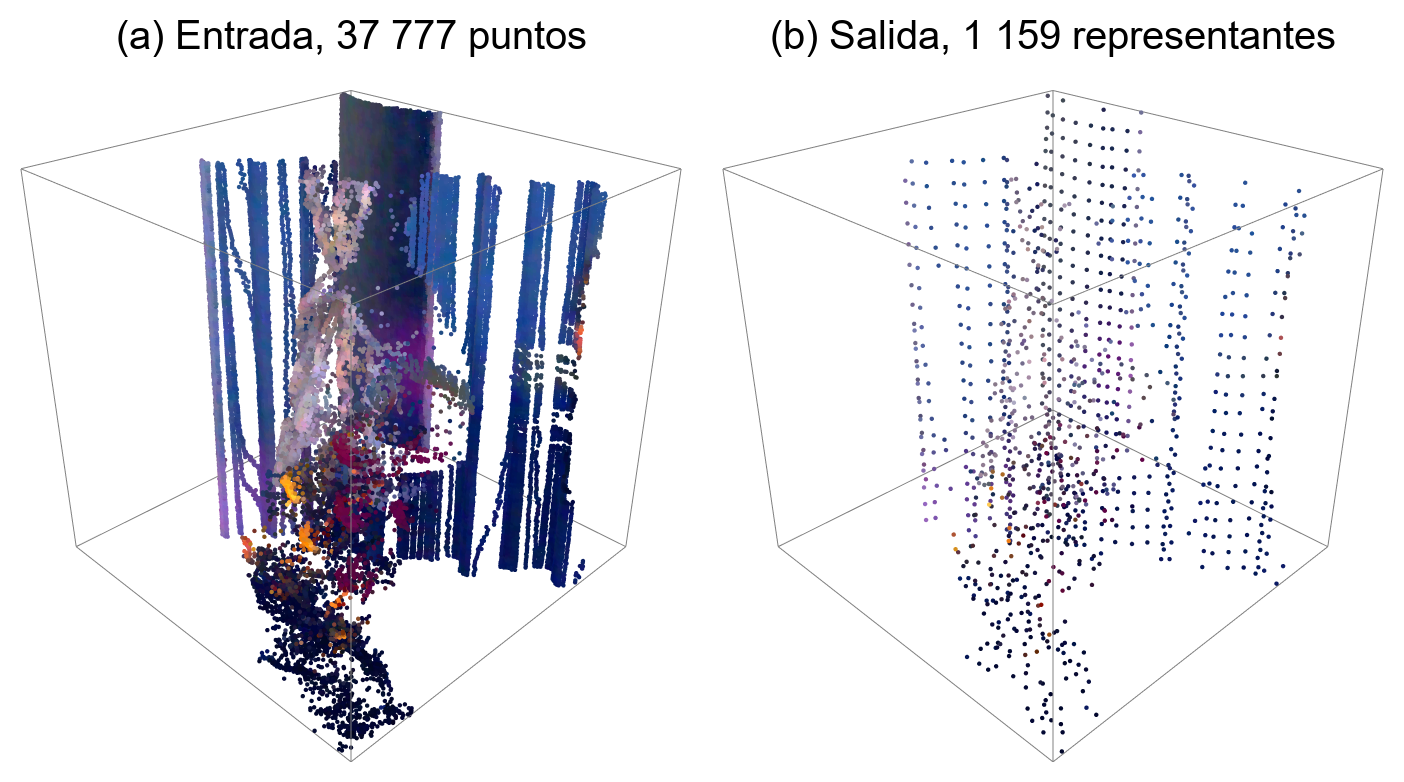
\includegraphics[width=0.6\linewidth]{imagenes/m1_paso4_voxel_cubo_pl13.png}
\caption[Cubo de 1\,m de PL13 antes y después de la voxelización]{Cubo de 1\,m de PL13 antes y después de la voxelización. Elaboración propia con el visor del proyecto (\hyperref[sec:anexo-software]{Anexo~A}).}
\label{fig:cubo-pl13}
\end{figure}

\begin{figure}[!htbp]
\centering
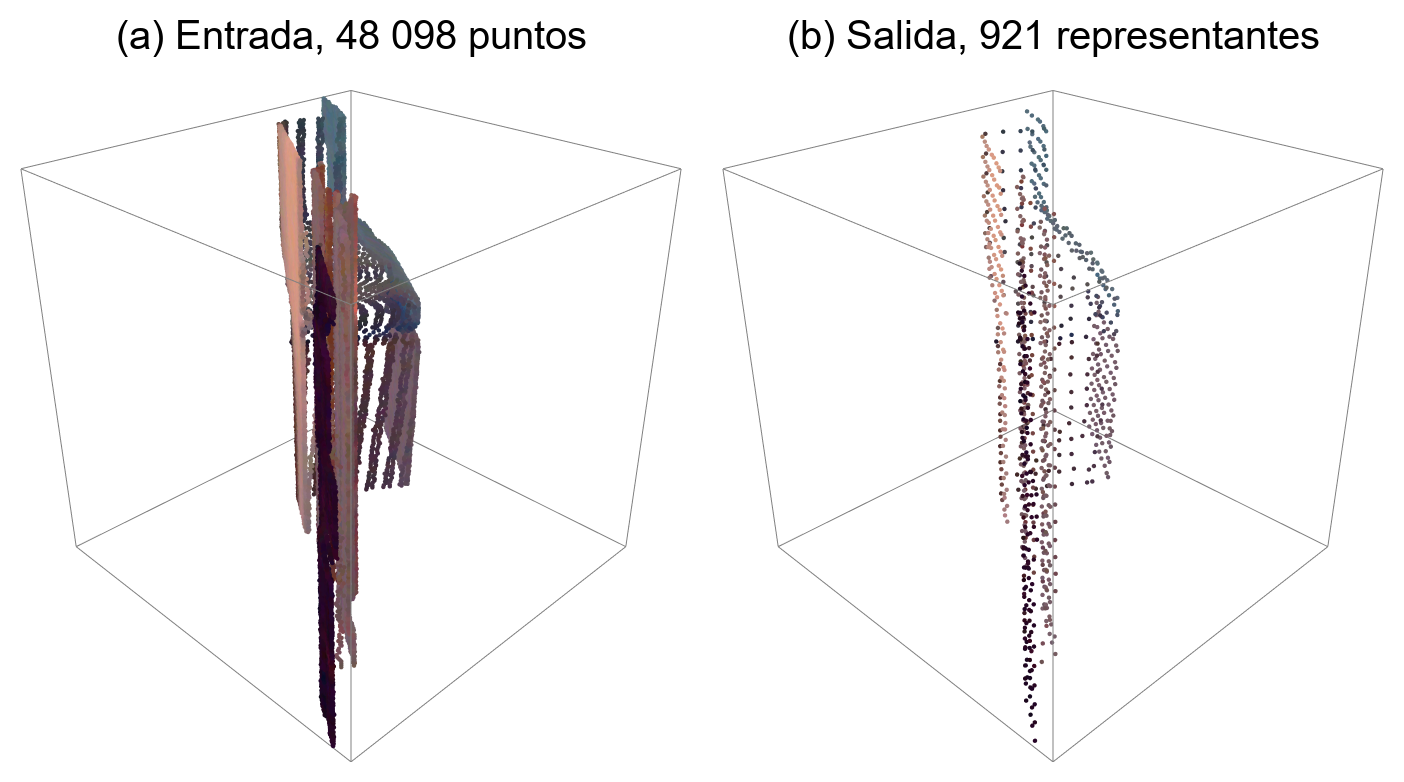
\includegraphics[width=0.6\linewidth]{imagenes/m1_paso4_voxel_cubo.png}
\caption[Cubo de 1\,m de PL7 antes y después de la voxelización]{Cubo de 1\,m de PL7 antes y después de la voxelización. Elaboración propia con el visor del proyecto (\hyperref[sec:anexo-software]{Anexo~A}).}
\label{fig:cubo-pl7}
\end{figure}

\FloatBarrier
\subsubsection*{Paso 5. Normales}

Las superficies con la misma orientación toman el mismo tono
(Figura~\ref{fig:m1-paso5}). En las bóvedas el
color cambia de forma gradual, siguiendo su curvatura. En las zonas ralas, lejos
del escáner, aparecen manchas de colores mezclados. Es la misma zona en la que el
filtrado del Paso~3 concentró sus descartes.

\begin{figure}[!htbp]
\centering
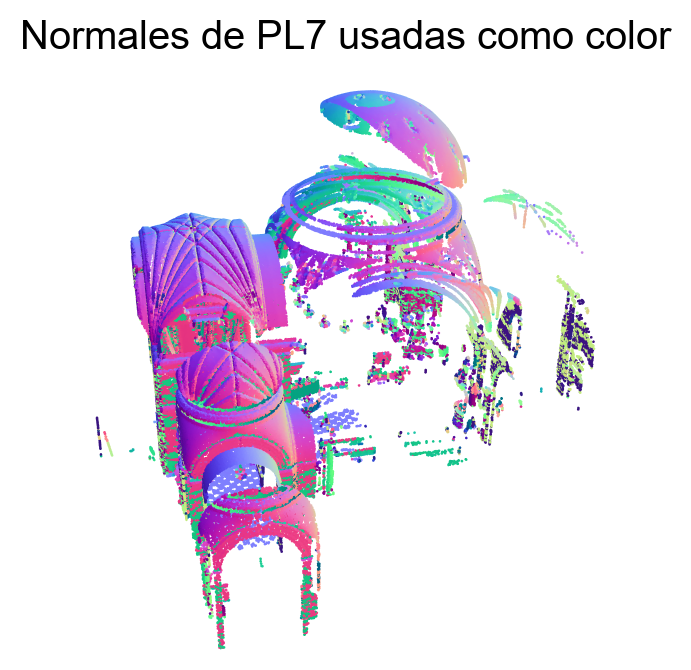
\includegraphics[width=0.75\linewidth]{imagenes/m1_paso5_normales.png}
\caption[Normales de PL13 y PL7 como color]{Normales de PL13 y PL7 como color. Elaboración propia con el visor del proyecto (\hyperref[sec:anexo-software]{Anexo~A}).}
\label{fig:m1-paso5}
\end{figure}

\FloatBarrier
\subsubsection*{Paso 6. Escritura}

En PL13 la matriz $S$ ocupa 28{,}9\,MB y en PL7 22{,}0\,MB, junto a su archivo de metadatos (Tabla~\ref{tab:m1-metadatos}).

\begin{table}[!htbp]
\centering
\setstretch{1}\small
\caption[Metadatos de PL13 y PL7]{Metadatos de PL13 y PL7. Los campos se describen en el Paso~6 de la Sección~\ref{sec:u1-procedimiento}. Elaboración propia.}
\label{tab:m1-metadatos}
\begin{tabularx}{\linewidth}{@{}l>{\raggedright\arraybackslash}X>{\raggedright\arraybackslash}X@{}}
\toprule
\textbf{Campo} & \textbf{PL13} & \textbf{PL7} \\
\midrule
\texttt{voxel} & 0{,}05 & 0{,}05 \\
\texttt{q} & 20 & 20 \\
\texttt{lambda} & 2 & 2 \\
\texttt{offset\_utm} & \multicolumn{2}{l}{Columna \emph{Centro} de la Tabla~\ref{tab:m1-centrado}} \\
\texttt{n\_crudo} & 8\,239\,904 & 8\,590\,904 \\
\texttt{n\_sor} & 8\,020\,796 & 8\,184\,419 \\
\texttt{n\_voxel} & 803\,099 & 610\,637 \\
\texttt{segundos} & 12{,}0 & 14{,}4 \\
\bottomrule
\end{tabularx}
\end{table}

\FloatBarrier
\subsection{Verificación y Reproducibilidad}
\label{sec:res-u1-repro}

Responde a la Sección~\ref{sec:u1-reproducibilidad}. PL13 se ejecutó con la
orden de esa sección y PL7 con la siguiente.
\begin{lstlisting}[style=comando]
python preprocesar.py --input PL7_SCN0001.las \
       --output PL7_SCN0001_preprocesado \
       --voxel 0.05 --q 20 --lam 2
\end{lstlisting}

El mismo programa preprocesó después el levantamiento completo en el clúster
Khipu, con los mismos parámetros. Los 23 archivos LAS
(Sección~\ref{sec:u1-datos}) quedaron en 17\,807\,859 representantes. La suma de los tiempos por
archivo fue de 1\,079 segundos, unos 18 minutos. Los conteos de PL13 y de PL7
en esa corrida coinciden exactamente con los de las pruebas locales de la
Tabla~\ref{tab:m1-metadatos}, que es la comprobación de repetición descrita en
la Sección~\ref{sec:u1-reproducibilidad}: la unidad da el mismo resultado en dos
máquinas distintas.

% =====================================================================
\FloatBarrier
\section{Unidad 2. Extracción de Descriptores y Fusión}
\label{sec:res-unidad2}

Responde a la Sección~\ref{sec:unidad2}.

\FloatBarrier
\subsection{Rama Semántica}

Responde a la Sección~\ref{sec:rama-sem}. No se ha ejecutado.

\FloatBarrier
\subsection{Rama Auto-supervisada Congelada}
\label{sec:res-rama-ssl}

Responde a la Sección~\ref{sec:rama-ssl}. Se ejecutó sobre PL13 en Khipu. En el clúster
el archivo se llama \texttt{PL13'\_SCN0001.las}, con apóstrofo, y el guion de
lanzamiento lo quita al nombrar la salida, que queda como
\texttt{PL13\_SCN0001}. La entrada fue la matriz $S$ de PL13 generada en Khipu
(Sección~\ref{sec:res-u1-repro}), en 15{,}8 segundos.


\FloatBarrier
\subsubsection*{Paso 1. Carga de la matriz}

Se leen 803\,099 filas en 0{,}3 segundos; es la salida del Paso~6 de la
Unidad~1 (Figura~\ref{fig:m3-paso1}).

\begin{figure}[!htbp]
\centering
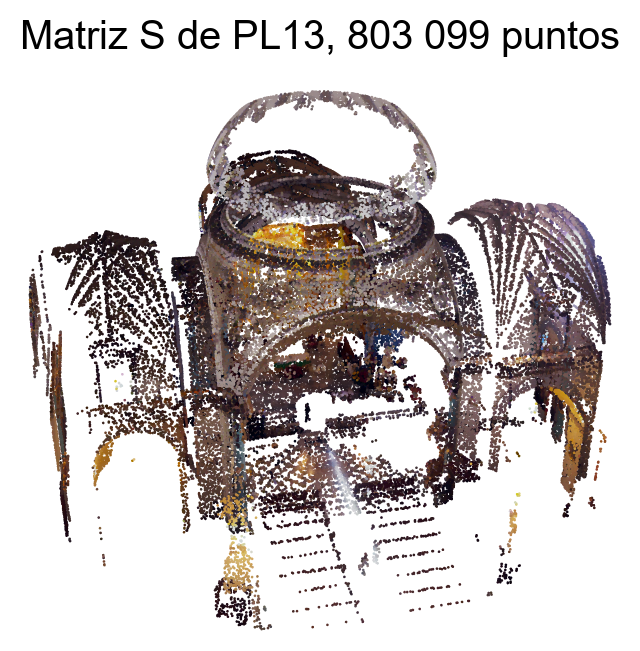
\includegraphics[width=0.4\linewidth]{imagenes/m3_paso1_entrada.png}
\caption[Matriz $S$ de PL13, entrada de Sonata]{Matriz $S$ de PL13, entrada de Sonata. Elaboración propia con el visor del proyecto (\hyperref[sec:anexo-software]{Anexo~A}).}
\label{fig:m3-paso1}
\end{figure}

\FloatBarrier
\subsubsection*{Paso 2. Carga del modelo}

El modelo cargado tiene 108{,}46 millones de parámetros, cifra que imprime la
función de carga de Sonata.

\FloatBarrier
\subsubsection*{Paso 3. Preparación}

La rejilla retiene casi todos los puntos (Tabla~\ref{tab:salidas-p2}). La
diferencia no se distingue a simple vista, por eso este paso no lleva imagen. La
causa es que el vóxel de 5\,cm de la
Unidad~1 ya dejó la nube más gruesa que la rejilla de Sonata, de modo que casi
toda celda contiene un solo punto.

\FloatBarrier
\subsubsection*{Paso 4. Inferencia}

El tiempo, el rendimiento y la memoria de la inferencia están en la
Tabla~\ref{tab:salidas-p2}. La Figura~\ref{fig:visor-pl13-etapas} muestra los
descriptores con la primera vista de la Sección~\ref{sec:revision-descriptores}.
Cada panel dibuja 100\,000 puntos al azar, por eso la
reducción de la Unidad~1 no se aprecia entre los dos primeros; se aprecia en la
Figura~\ref{fig:m1-paso4-pl13}.

\begin{figure}[!htbp]
\centering
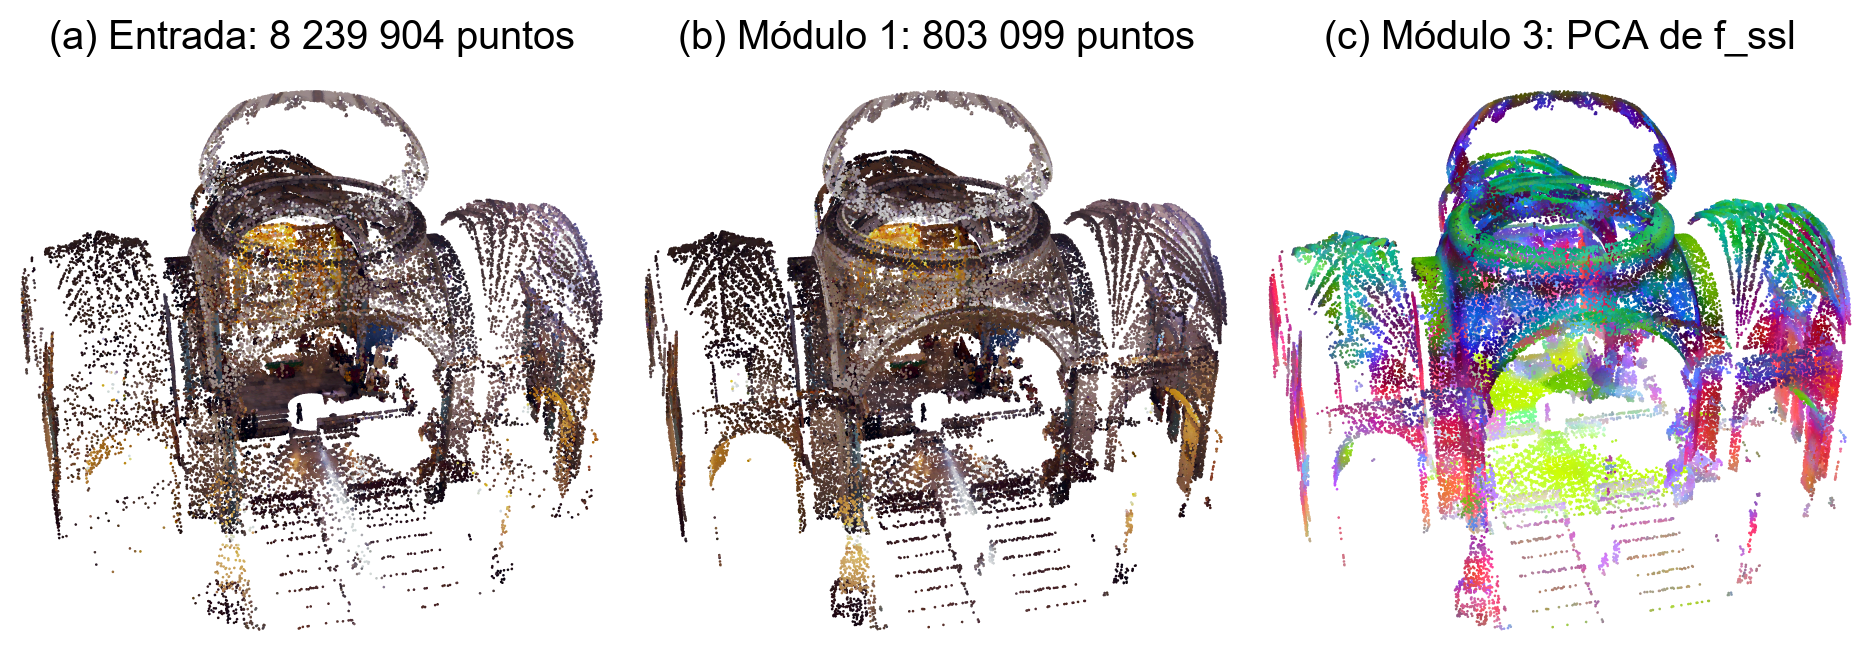
\includegraphics[width=0.8\linewidth]{imagenes/visor_pl13_entrada_m1_m3.png}
\caption[PL13 en sus tres etapas]{PL13 crudo, tras la Unidad~1 y con los descriptores de Sonata. Elaboración propia con el visor del proyecto (\hyperref[sec:anexo-software]{Anexo~A}).}
\label{fig:visor-pl13-etapas}
\end{figure}

\FloatBarrier
\subsubsection*{Paso 5. Escritura}

El contenido del archivo \texttt{.npz} está en la Tabla~\ref{tab:npz} y su
tamaño en la Tabla~\ref{tab:salidas-p2}. Tiene cinco
campos y no seis porque esta extracción se hizo antes de que el programa
guardara la semilla.

\begin{table}[!htbp]
\centering
\setstretch{1}\small
\caption[Archivo de descriptores de PL13]{Archivo de descriptores de PL13. Los campos se describen en el Paso~5 de la Sección~\ref{sec:rama-ssl}. Elaboración propia.}
\label{tab:npz}
\begin{tabular}{@{}ll@{}}
\toprule
\textbf{Campo} & \textbf{Valor en PL13} \\
\midrule
\texttt{feat} & $796\,315\times 1088$, precisión media \\
\texttt{coord} & $796\,315\times 3$ \\
\texttt{inverse} & $803\,099$ entradas \\
\texttt{grid\_size} & 0{,}02\,m \\
\texttt{n\_original} & 803\,099 \\
\bottomrule
\end{tabular}
\end{table}

\FloatBarrier
\subsubsection*{Observables}
\label{sec:res-observables}

Responde a la Sección~\ref{sec:observables} (Tabla~\ref{tab:salidas-p2}).

\begin{table}[!htbp]
\centering
\setstretch{1}\small
\caption[Observables de Sonata en PL13: esperado y medido]{Observables de Sonata en PL13: esperado y medido. Para qué sirve cada uno se explica en la Sección~\ref{sec:observables}. Elaboración propia.}
\label{tab:salidas-p2}
\begin{tabularx}{\linewidth}{@{}>{\raggedright\arraybackslash}Xll@{}}
\toprule
\textbf{Observable} & \textbf{Esperado} & \textbf{Medido} \\
\midrule
Dimensión de $f_{\mathrm{ssl}}$ & 1088 & 1088 \\
Puntos retenidos tras el muestreo por rejilla & --- & 796\,315 de 803\,099, el 99{,}2\,\% \\
VRAM pico & Cota de 4{,}2\,GB & 34{,}60\,GB \\
Tiempo de inferencia por sección & --- & 13{,}9\,s \\
Rendimiento en puntos por segundo & --- & 57\,397 \\
Tamaño del archivo de descriptores & --- & 680\,MB \\
\bottomrule
\end{tabularx}
\end{table}

La memoria es el observable que más se aparta de lo esperado. La cota de
4{,}2\,GB se calculó para una sección de $3\times10^{5}$ puntos, y PL13 entró a
Sonata con 796\,315, unas 2{,}7 veces más, por lo que las dos cifras no se
comparan directamente. Lo que sí indica la medición es cuánto margen queda: una
sección de unos $8\times10^{5}$ puntos ocupa el 72\,\% de los 48\,GB de la GPU.
Ese es el dato con que se planificarán las secciones mayores, en lugar de la
cota.

\FloatBarrier
\subsubsection*{Revisión de los descriptores}
\label{sec:res-descriptores}

Responde a la Sección~\ref{sec:revision-descriptores}. La primera vista, las
componentes principales, es el tercer panel de la
Figura~\ref{fig:visor-pl13-etapas}; las otras dos están en la
Figura~\ref{fig:sonata-pl13}, desde la misma cámara.

\begin{figure}[!htbp]
\centering
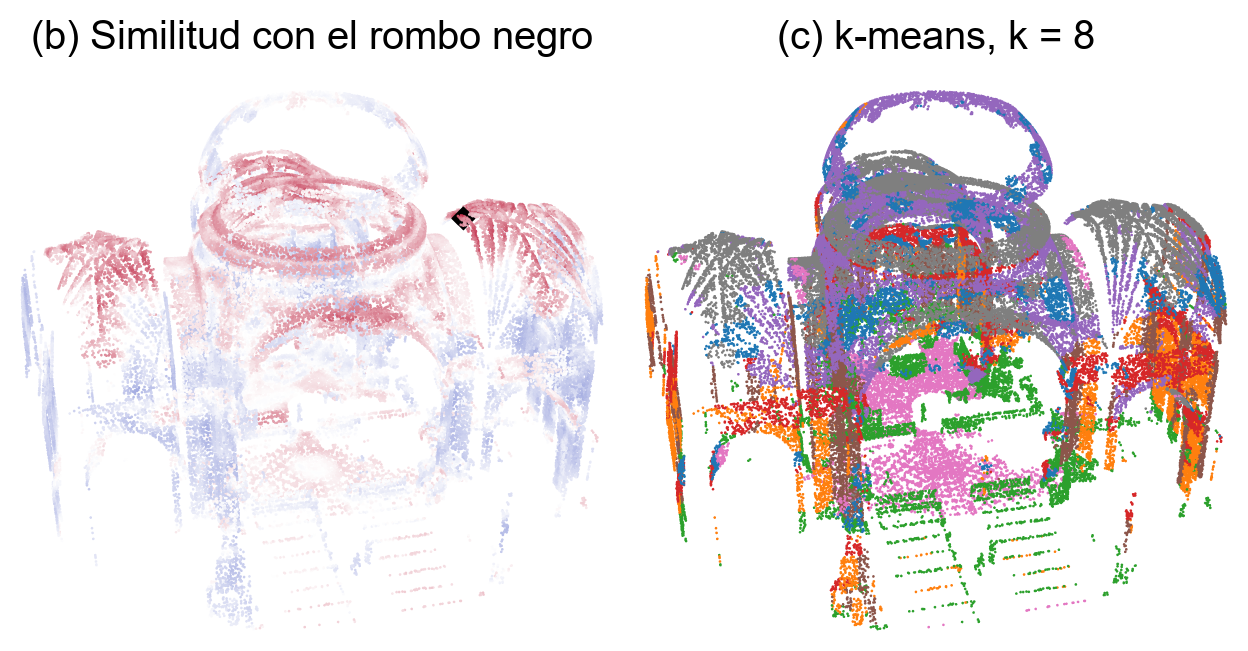
\includegraphics[width=0.6\linewidth]{imagenes/visor_pl13_descriptores_m3_sin_pca.png}
\caption[Similitud y $k$-means de los descriptores de PL13]{Similitud y $k$-means de los descriptores de PL13. Elaboración propia con el visor del proyecto (\hyperref[sec:anexo-software]{Anexo~A}).}
\label{fig:sonata-pl13}
\end{figure}

Sobre la misma muestra, las tres primeras componentes principales explican el
25{,}3\,\% de la varianza, las diez primeras el 43{,}4\,\% y el rango efectivo
es de 110{,}6 sobre 1088 dimensiones. Esto significa dos cosas. La primera es que
el color de la vista de componentes principales, que usa solo tres, muestra una
cuarta parte de la información de los descriptores; dos puntos del mismo color
pueden diferir en el resto. La segunda es que los descriptores no han colapsado:
el rango efectivo valdría 1 si todos apuntaran en la misma dirección
(Sección~\ref{sec:revision-descriptores}), y equivale aquí a unas 110
direcciones independientes.

\FloatBarrier
\subsection{Punto de Fusión}

Responde a la Sección~\ref{sec:fusion}. No se ha ejecutado.

% =====================================================================
\FloatBarrier
\section{Justificación de los Parámetros del Procedimiento}
\label{sec:res-parametros}

Responde a la Sección~\ref{sec:parametros}. Las pruebas P0 a P5 aún no se han
ejecutado, de modo que los valores usados en las Secciones~\ref{sec:res-unidad1}
y~\ref{sec:res-unidad2} son los que trae el programa por defecto. Lo ejecutado
de esta sección son dos comprobaciones.

\paragraph*{Efecto de cada paso.} Los efectos que la
Sección~\ref{sec:param-funcion} atribuye a cada paso se observan en las salidas:
el descarte del filtrado en las zonas ralas (Figura~\ref{fig:m1-paso3}), la
pérdida de superficies próximas por el vóxel (Figura~\ref{fig:cubo-pl7}), las
normales ruidosas de las zonas ralas (Figura~\ref{fig:m1-paso5}) y la retención
casi total de la rejilla de Sonata (Tabla~\ref{tab:salidas-p2}).

\paragraph*{Replicación.} Responde a la Sección~\ref{sec:param-replicacion}. La
replicación de la configuración de referencia está en la
Sección~\ref{sec:res-u1-repro}.

% =====================================================================
\FloatBarrier
\section{Unidad 3. Entrenamiento, Calibración y Evaluación}
\label{sec:res-unidad3}

Responde a la Sección~\ref{sec:unidad3}. Esta unidad aún no se ha ejecutado.
Lo único hecho es la verificación del entorno de la
Sección~\ref{sec:entorno-computo}: con MinkowskiEngine compilado, una corrida de
HyperNCD en Khipu llegó hasta la carga del primer lote.

% =====================================================================
\FloatBarrier
\section{Riesgos y Mitigación}

Responde a la Sección~\ref{sec:riesgos}.

\paragraph*{(i) Disponibilidad de la nube anotada.} El riesgo se materializó: los
23 archivos LAS llegaron sin etiquetas (Sección~\ref{sec:u1-datos}), así que se
aplica la mitigación prevista.

\paragraph*{(ii) Acceso y configuración del clúster.} Verificado: la Unidad~2
corrió en la GPU asignada (Sección~\ref{sec:res-hardware}).

% =====================================================================
\FloatBarrier
\section{Resumen de los Resultados Preliminares}

Responde a la Sección~\ref{sec:conclusion-metodo}. Las Unidades~1 y~2 se
ejecutaron paso a paso sobre escaneos reales y cada paso entregó la salida que
declara la metodología; la Unidad~1 se reprodujo en otra máquina
(Sección~\ref{sec:res-u1-repro}). Son resultados preliminares: muestran que el
procedimiento funciona y se repite, no todavía que mejore la segmentación.
